In the previous chapter, we have introduced the ShICA model, a principled
unifying solution to the problems of shared response
modeling and GroupICA. In this chapter we evaluate its practical utility on
synthetic data and on brain imaging data.

\section{Synthetic experiment}
In the following synthetic experiments, data are generated according to model~\eqref{eq:model} with $p=4$ components and $m=5$ views and mixing matrices are generated by sampling coefficients from a standardized Gaussian.
\subsection{Separation performance: different use cases}
\label{sec:rotation}
%\pierre{Make sure that algos are always in the same order in legend, and that shica-j and shica ml are together}
Gaussian components are generated from a standardized Gaussian and their noise
has standard deviation $\Sigma_i^{\frac12}$ where $\Sigma_i^{\frac12}$ is a
[Omitted long matching line]
\begin{figure}
\centering
  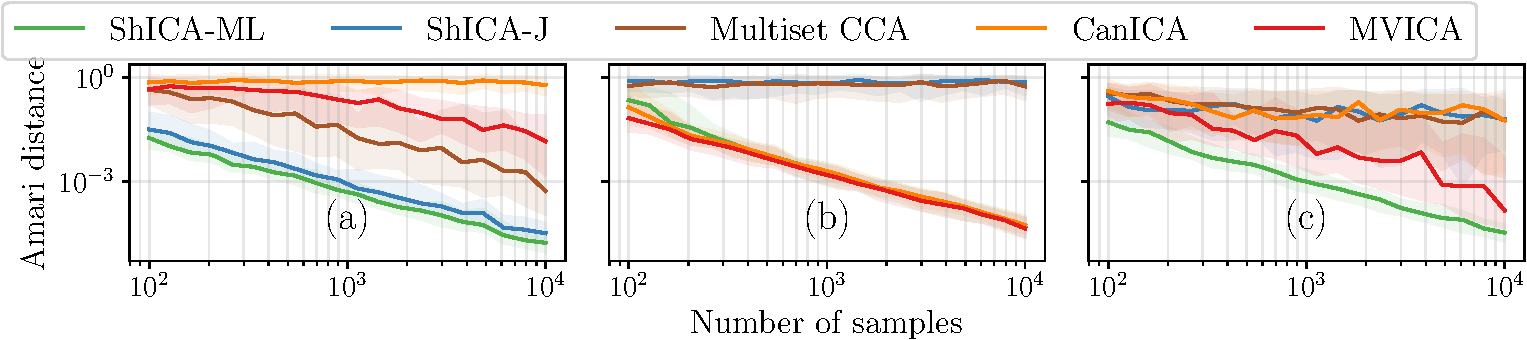
\includegraphics[width=0.9\textwidth]{./figures/amvica/identifiability.pdf}
  \caption{\textbf{Separation performance}: Algorithms are fit on data following model~\ref{eq:model} \textbf{(a)} Gaussian components with noise diversity \textbf{(b)} Non-Gaussian components without noise diversity \textbf{(c)} Half of the components are Gaussian with noise diversity, the other half is non-Gaussian without noise diversity. 
  %\aapo{[It would be nice to have labels a,b,c but this is not critical.]}
  %\Alex{Make the legend fit on one line and rename Multiset CCA to Multiset CCA to be consistent with the text (or update text). Also you should be able to reduce a tiny bit the height of the axes plots.}
  }
  \label{exp:rotation}
\end{figure}
When all components are Gaussian (Fig.~\ref{exp:rotation}~(a)), CanICA cannot
separate the components at all. In contrast ShICA-J, ShICA-ML and Multiset CCA
are able to separate them, but Multiset CCA needs many more samples to reach the
same Amari distance as ShICA-J or ShICA-ML, which shows that correcting for the
rotation due to sampling noise improves the results. Looking at error bars, we
also see that the performance of Multiset CCA varies quite a lot with the random
seeds: this shows that depending on the sampling noise, the rotation can be very
different from identity. MultiViewICA does achieve separation but obtains
relatively poor separation performance compared to ShICA or Multiset CCA.
When none of the components are Gaussian (Fig.~\ref{exp:rotation}~(b)), only
CanICA, ShICA-ML and MultiView ICA are able to separate the components, as other methods do not make use of non-Gaussianity.
Finally, in the hybrid case (Fig.~\ref{exp:rotation}~(c)), ShICA-ML is able to
separate the components very well as it can make use of both non-Gaussianity and
noise diversity. As we can see, MultiView ICA yields decent performance though
uniformly worse than ShICA-ML. Also note that error bars are very large showing
that for some seeds it gives poor results. Overall, MultiView ICA is a lot less
reliable than ShICA-ML.


\subsection{Separation performance in function of non-Gaussianity}
We generate data according to model~\eqref{eq:model}. Components $\sbb$ are
generated using $s_j = d(x)$ with $d(x) = x |x|^{\alpha - 1}$ and $x \sim
\mathcal{N}(0, 1)$. We impose noise diversity: the noise of view $i$ has standard deviation $\Sigma_i^{\frac12}$ (obtained by sampling from a uniform density between $0$ and $1$).
[Omitted long matching line]
 When $\alpha$ is close to 1 (components are almost Gaussian), ShICA-J, ShICA-ML and multiset CCA can separate components well (but multiset CCA reaches higher Amari distance than ShICA). In this regime, MultiViewICA yields much higher Amari distance than ShICA-J, ShICA-ML or Multiset CCA but is still better than CanICA which cannot separate components at all.
 As non-Gaussianity ($\alpha$) increases, ICA based methods yield better results but ShICA-ML yields uniformly lower Amari distance.
\begin{figure}
\centering
  \includegraphics[width=0.8\textwidth]{./figures/amvica/synthetic_Gaussian_source.pdf}
  \caption{\textbf{ Separation performance in function of non-Gaussianity} Separation performance of algorithms for sub-Gaussian $\alpha < 1$ and super-Gaussian $\alpha > 1$ components}
  \label{exp:separatingpower}
\end{figure}

\subsection{Computation time}
\begin{figure}
    \centering
    \includegraphics[width=.65\linewidth]{./figures/amvica/synthetic_Gaussian_timings.pdf}
    \caption{\textbf{Computation time: } Algorithms are fit on data generated from model~\eqref{eq:model} with a super-Gaussian density. For different values of the number of samples, we plot the Amari distance and the fitting time. Thick lines link median values across seeds.}
    \label{exp:syn_timings}
\end{figure}
[Omitted long matching line]
%


%\pierre{fig might have a smaller legend: 3 cols, smaller fonts}


% The difference between AVICA and other approaches can be quantified via a
% statistical t-test on the difference of log distances. It
% gives the p-values $4.57 \times 10^{-4}$, $5.93 \times 10^{-4}$ and $2.37
% \times 10^{-9}$ w.r.t.
% MVICA, PermICA and ConcatICA respectively.
\section{Experiments on brain imaging data}

\subsection{Robustness w.r.t intra-subject variability in MEG}
\begin{figure}
  \centering
  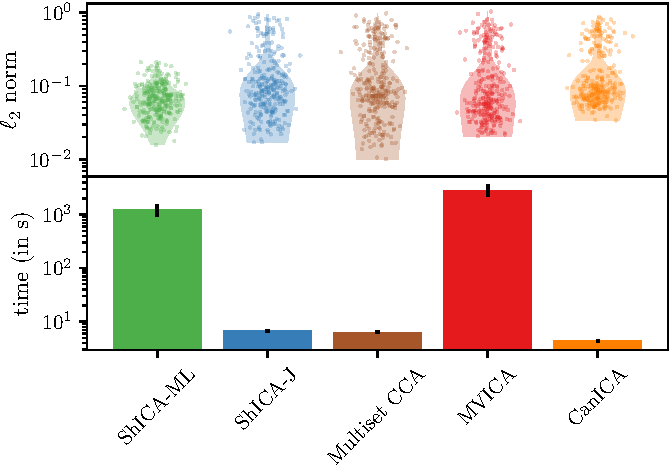
\includegraphics[width=.65\linewidth]{./figures/amvica/inter_subject_stability.pdf}
  \caption{\textbf{Robustness w.r.t intra-subject variability in MEG}:
    (\textbf{top}) $\ell_2$ distance between shared components corresponding to the same stimuli in different trials.  (\textbf{bottom}) Fitting time.
    %\Alex{Should be $\ell_2$ in ylabel not L2}
}
\label{fig:eeg_intragroup_variability}
\end{figure}
In the following experiments we consider the Cam-CAN
dataset~\cite{taylor2017cambridge}. We use the magnetometer data from the MEG of $m=100$ subjects chosen randomly among 496.
% 
Each subject is repeatedly presented three audio-visual stimuli. 
% 
For each stimulus, we divide the trials into two sets and within each set, %Aapo: "sets"
the MEG signal is averaged across trials to isolate the evoked response. This
procedure yields 6 chunks of individual data (2 per stimulus).
%
% The 6 chunks of data are concatenated in the time direction and ICA algorithms
% are applied separately to extract $k=10$ shared components that we plot in
% appendix~\ref{megcomponents} and localize in appendix~\ref{megcomponentslocal}.
%
We study the similarity between shared components corresponding to repetitions of the same stimulus. This gives a measure of robustness of each ICA algorithm with respect
to intra-subject variability.
Data are first reduced using a subject-specific PCA with $p=10$ components. Algorithms are run 10 times with different seeds on the 6 chunks of data,
and shared components are extracted.
%
When two chunks of data correspond to repetitions of the same stimulus they should yield similar
components.
%
For each component and for each stimulus, we therefore measure the $\ell_2$
distance between the two repetitions of the stimulus.
 This yields $300$ distances per algorithm that are
plotted on Fig~\ref{fig:eeg_intragroup_variability}.

The components recovered by ShICA-ML have a much lower variability than other approaches. The performance of ShICA-J is competitive with Multiview ICA while being much faster to fit. Multiset CCA yields satisfying results compared with ShICA-J. However we see that the number of components that do not match at all across trials is greater in Multiset CCA.

The mixing operators in ShICA define spatial maps. In appendix~\ref{app:shica:maps}, we plot
the average spatial maps across subjects.

    %\bt{Muliview ICA appears only now ?} \aapo{[Actually, multiset CCA looks just as good as ShICA-J?, comments?.]}

\subsection{MEG Phantom experiment}
\label{app:phantom}
\subsubsection{Elekta Phantom}
We use the \emph{Elektra Phantom MEG} dataset described
in~\ref{sec:meg:datasets} where dipoles at $m=32$ different locations emit the
same signal.
    We reduce the data by applying view specific PCA with $k=20$ components and algorithms are applied on the reduced data. We select the component that is closer to the true one and compute the L2 norm between the predicted component and the true one after normalization.
    Then we attempt to recover the position of each dipole by performing dipole fitting on the mixing operator of each view (using only the column corresponding to the true component). The localization error is defined as the mean l2 distance between the true localization and the predicted localization where the mean is computed across dipoles. 
    Each epoch corresponds to 301 samples and 20 epochs are available in total. We vary the number of epochs between 2 and 18 and display in Fig~\ref{exp:meg_phantom} the reconstruction error and the localization error as a function of the number of epochs used.
    ShICA-ML outperforms other methods. ShICA-J gives satisfying results while being much faster.
    
    \subsubsection{MEG Phantom Sinusoidal components}
    We reproduce the phantom experiment presented in section~\ref{sec:mvica:phantom}. ShICA-ML outperforms other methods. ShICA-J gives satisfying results while being much faster.
    
\begin{figure}
\centering
  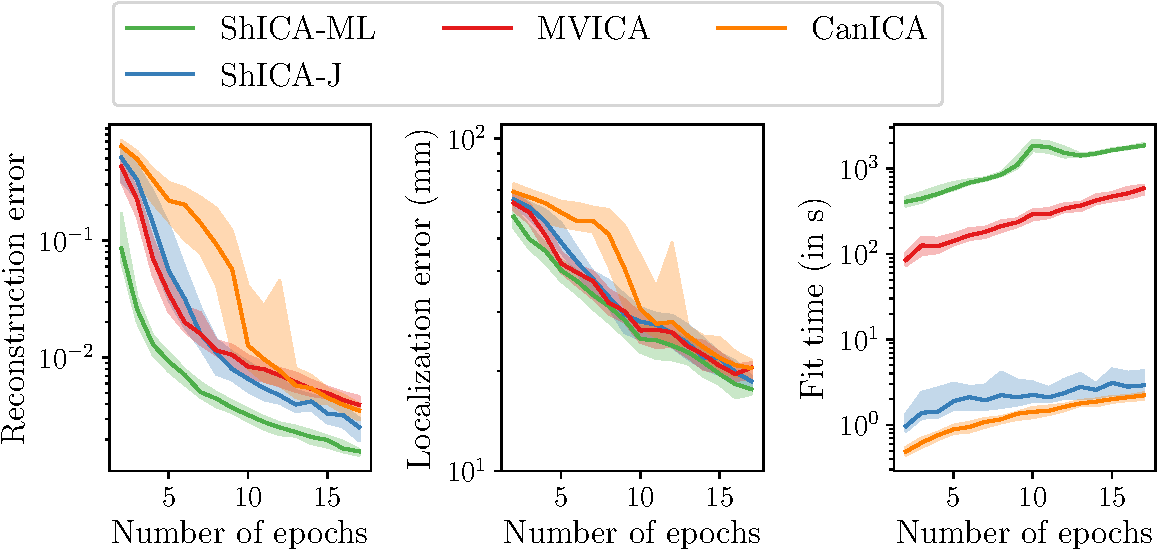
\includegraphics[width=0.9\textwidth]{./figures/amvica/meg_phantom.pdf}
  \caption{\textbf{MEG Phantom (Elekta)}: (left) L2 distance between the predicted and actual component (middle) Mean error (in mm) between predicted and actual dipoles localization (right) Fitting time (in seconds)}
\label{exp:meg_phantom}
\end{figure}

\begin{figure}
\centering
  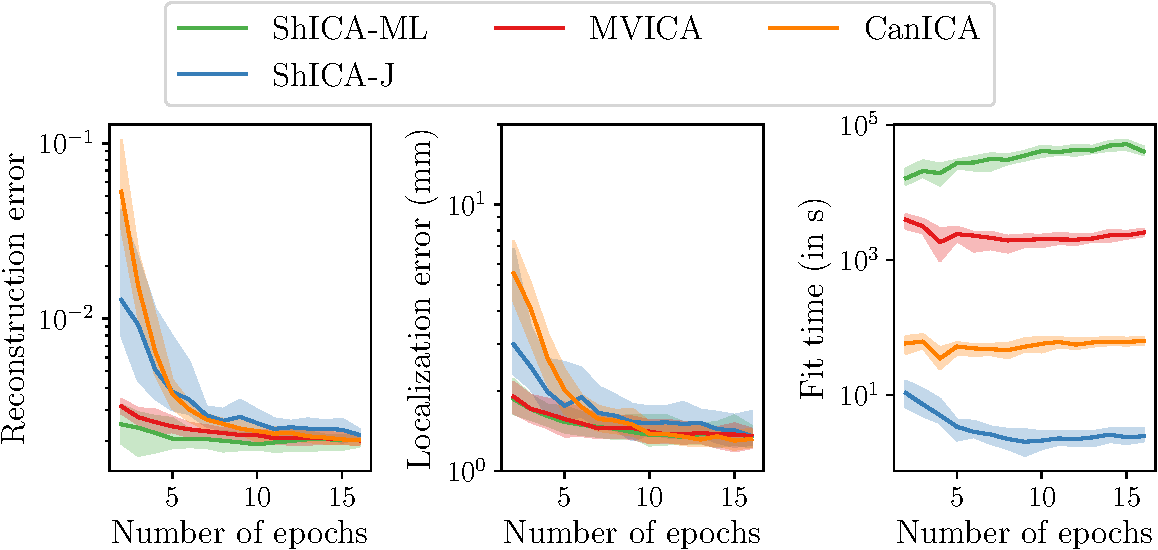
\includegraphics[width=0.9\textwidth]{./figures/amvica/meg_phantom_neurips.pdf}
  \caption{\textbf{MEG Phantom Sinusoidal components}: (left) L2 distance between the predicted and actual component (middle) Mean error (in mm) between predicted and actual dipoles localization (right) Fitting time (in seconds)}
\label{exp:meg_phantom_neurips}
\end{figure}



\subsection{Reconstructing the BOLD signal of missing subjects}
\begin{figure}
  \centering
  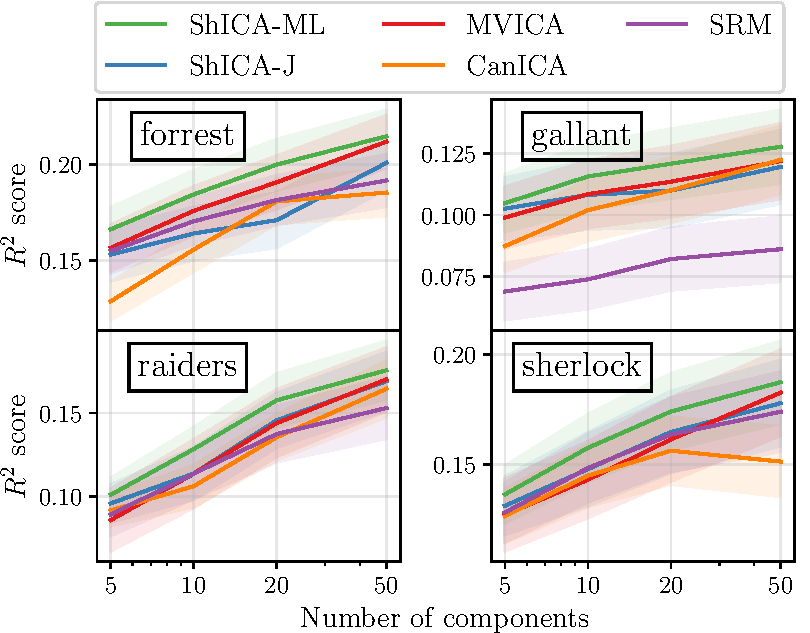
\includegraphics[width=0.49\linewidth]{./figures/amvica/reconstruction.pdf}
  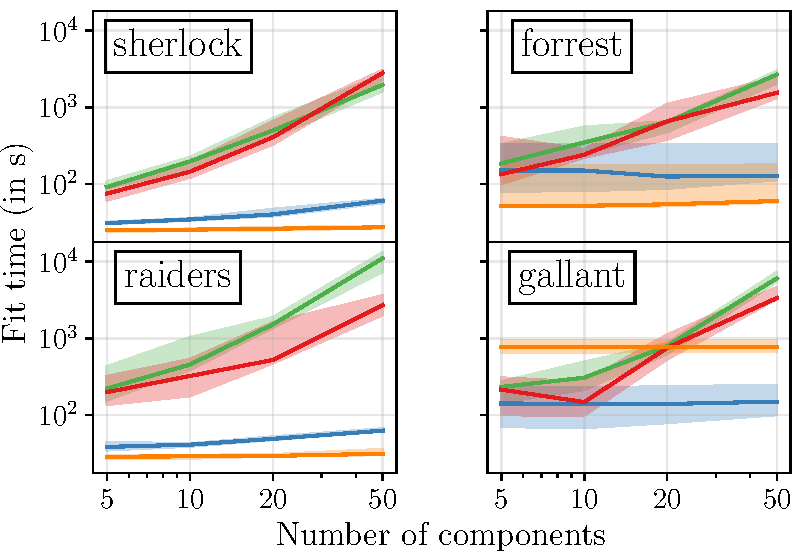
\includegraphics[width=0.49\linewidth]{./figures/amvica/reconstruction_timings.pdf}
  
  \caption{\textbf{Reconstructing the BOLD signal of
      missing subjects}. (\textbf{left}) Mean $R^2$ score between reconstructed data and true
    data. (\textbf{right}) Fitting time.
    %\Alex{ylabel should be $R^2$ not R2}
    }
  \label{fig:reconstruction}
\end{figure}

We reproduce the experiental pipeline described in section~\ref{sec:srm:reconstruction}.
ShICA-ML yields the best $R^2$ score in all datasets and for any number of
components. ShICA-J yields competitive results with respect to Multiview ICA
while being much faster to fit.


\subsection{fMRI timesegment matching experiment}
A popular benchmark especially in the SRM community is the time-segment matching
experiment~\cite{chen2015reduced} which we describe in
section~\ref{timesegment_expe}.
The left panel in Fig~\ref{exp:timesegment} shows that ShICA-ML, MultiViewICA and ShICA-J yield almost equal accuracy and outperform other methods by a large margin. The right panel in Fig~\ref{exp:timesegment} shows that ShICA-J is much faster to fit than MultiViewICA or ShICA-ML.


\begin{figure}
    \centering
    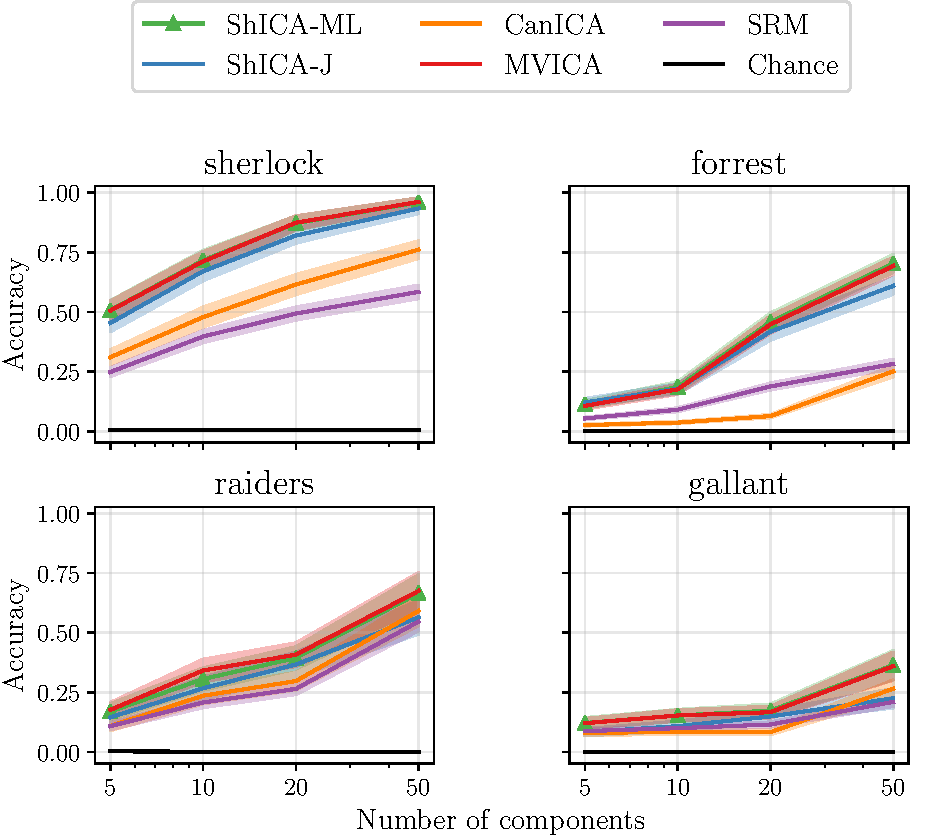
\includegraphics[width=0.49\textwidth]{./figures/amvica/timesegment_matching.pdf}
    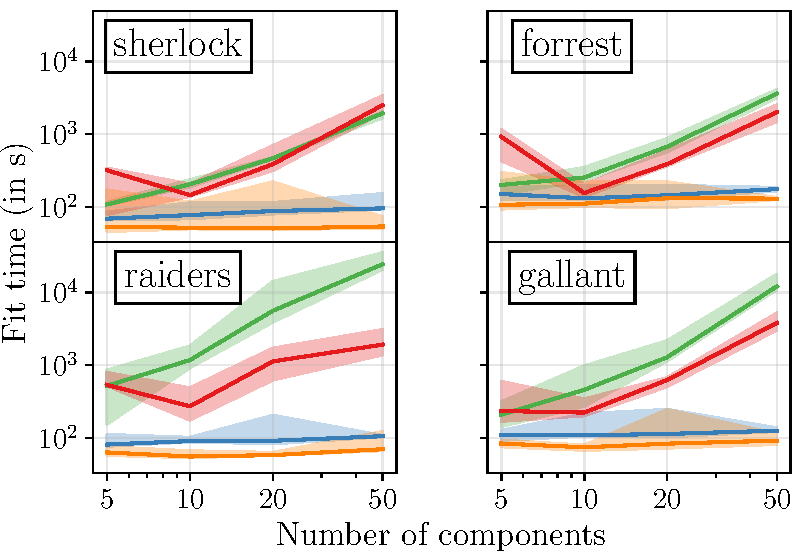
\includegraphics[width=0.49\textwidth]{./figures/amvica/timesegment_matching_timings.pdf}
    \caption{\textbf{Timesegment matching experiment}: (left) Accuracy (right) Fitting time (in seconds)}
    \label{exp:timesegment}
\end{figure}

% AVICA exhibits a small improvement on sherlock and raiders datasets that is
% consistent for different numbers of components (i.e. numbers of components) and competitive results on clips and forrest datasets.

% 

%\pierre{right plot is hard to read, too wide. Lots of space to gain here}

\section{Conclusion}
In this chapter, we have shown the practical benefits of ShICA.
On simulated data, ShICA clearly outperforms all competing methods in terms of the trade-off between statistical accuracy and computation time. On brain imaging data, ShICA gives more stable decompositions for comparable computation times, and more accurately predicts the data of one subject from the data of other subjects, making it a good candidate to perform transfer learning.
%ShICA inherits the ethical questions linked to its field of application.
As ShiCA only involves linear transforms, decisions based on its output are easier to interpret, making it accessible to practitioners.
%This work can help in brain disease diagnosis and reduce their human and societal burden.

In the next section, we show that ICA can be used to perform data augmentation
in fMRI.

% \section{A fast two-step approach for MIFA}

% While maximum-likelihood approaches possess several important statistical properties that make them attractive, a major drawback is the slowness of the algorithms. 
% %
% These method also require the likelihood to be well defined, and prevents dimension reduction without a more complicated model: for the likelihood to be well defined, we must assume that $A_i$ is square, invertible.
% Instead, we propose a two steps ad-hoc method, based on the following observations that were used for proving identifiability:
% \begin{itemize}
%     \item The knowledge of the empirical covariances $C_{ij}$ for $i\neq j$ allows to recover the mixing matrices $A_i$ up to a global rotation matrix.
%     \item Then, the knowledge of the ``diagonal'' terms $C_{ii}$ allows to eliminate this indeterminacy
% \end{itemize}
% These observations lead to the following two step approach
% \paragraph{Dimension reduction and global estimation}
% We first estimate jointly all the mixing matrices up to a global rotation by minimizing the criterion $\mathcal{L}(A_1, \dots, A_m) = \sum_{i \neq j} \|A_iA_j^{\top} - C_{ij}\|_F^2$.
% Since this cost function is quadratic with respect to each $A_i$, it is easily minimized w.r.t. one of the variable when all others are fixed:

% $$
% \arg\min_{A_i}\mathcal{L}(A_1\dots, A_m) = \left(\sum_{j\neq i} C_{ij}A_j\right)\left(\sum_{j\neq i}(A_j)^{\top}A_j\right)^{-1}
% $$
% Importantly, this formula also holds when the problem is over-determined, i.e. when $A_i\in \mathbb{R}^{p\times d}$ with $d < p$.
% We can then loop over all coordinates several times to obtain a block-coordinate descent algorithm. Each iteration of the algorithm is guaranteed to decrease the loss function. 
% The following lemma shows that minimizing the cost function leads to estimates of the true mixing matrices up to a global indeterminacy.
% \begin{proposition}
% Assume that for $i\neq j$, $C_{ij}= B_iB_j^{\top}$ for some matrices $(B_i)_{i=1}^m\in\mathbb{R}^{p\times d}$ with $d< p$. Then, $\mathcal{L}(A_1, \dots, A_m) = 0$ if and only if there exists $U\in\mathcal{O}_d$ such that $A_i = B_i U$ for all $i$.
% \end{proposition}
% {\textcolor{red}{Can we say anything about the algorithm ?  does it reach a local / global minimum?}}
% As a consequence, minimizing the previous criterion allows to reduce the dimension of the data. Importantly, since the problem is non-convex, we have no guarantee that the proposed algorithm reaches a global optimum. In practice, we found the proposed method to be robust.
% The last part of the procedure estimates the global rotation $U$ using joint diagonalization.
% \paragraph{Estimation of the global rotation by joint-diagonalization}
% We use the following property to estimation the global rotation.
% \begin{proposition} Assume that $C_{ii} = B_i(I_d + D_i)B_i^{\top}$ with $D_i$ a diagonal matrix with positive entries. Let $U$ an  orthogonal matrix, and $A_i = B_i U$, and $K_i = A_i^{-1}C_{ii}A_i^{-\top}$. Then, $U$ is a joint-diagonalizer of the set $K_i$, i.e. the matrices $U^{\top}K_i U$ are all diagonal.
% \end{proposition}
% Therefore, letting $A_i$ the outputs of the previous algorithms, we form the matrices $K_i$, and estimate the global rotation $U$ by joint-diagonalization of the $K_i$. The estimate of the mixing matrix is then $A_i U^{\top}$.
